\documentclass[a4paper, 12pt]{article}

% debug layout
%\usepackage{showframe}

% titles
\usepackage{titlesec}
% clickable urls
\usepackage[hyphens]{url}
% captions
\usepackage{caption}
\usepackage{subcaption}
% figures placement
\usepackage{float}
\usepackage{wrapfig}
% import images
\usepackage{graphicx}
\usepackage[export]{adjustbox}
% source code
\usepackage{listings}
% margins
\usepackage[a4paper,includeheadfoot,margin=2cm,top=5mm,head=47.5pt]{geometry}
% headers
\usepackage{fancyhdr}
\fancypagestyle{plain}{
    \fancyhf{}%
    \fancyhead[L]{\hspace{-15mm}
\includegraphics[height=1.5cm]{res/sjf_logo}}%
    \fancyfoot[C]{\thepage}%
    \renewcommand{\headrulewidth}{0pt}%
    \renewcommand{\footrulewidth}{0pt}%
}
\pagestyle{plain}
% fonts
\usepackage[T1]{fontenc}
\usepackage{helvet}
\renewcommand{\familydefault}{\sfdefault} % use sans-serif font

% change title style
\usepackage{titling}
\setlength{\droptitle}{-4em}
\pretitle{%
    \begin{flushleft}
    \setlength{\parindent}{0pt} %
    \Large \textbf{PROJECT REPORT} \\ %
    STUDY WEEK "FASCINATING INFORMATICS" \vspace{8pt} \\ \bf%
}
\posttitle{\end{flushleft}}

\preauthor{%
    \begin{flushleft}%
    \setlength{\parindent}{0pt} %
    %\begin{tabular}[t]{l}%
}
\postauthor{%
    %\end{tabular}%
    \vskip 1em%
    \textsuperscript{1}Kantonsschule Büelrain, Winterthur, Switzerland, %
    \textsuperscript{2}Scuola Arti e Mestieri Bellinzona, Ticino, Switzerland,%
    \textsuperscript{3}Kantonsschule Wattwil, St. Gallen, Switzerland. %
    \\ %
    \vskip 0.5em%
    Supervised by: Dominik Link%
    \end{flushleft}%
}
 
\predate{%
    \raggedleft%
    \setlength{\parindent}{0pt}%
    Date:%
}
\postdate{}

\title{Game Platform Mastermind}
\author{%
    Lukas Meili\textsuperscript{1}, %
    Naoki Pross\textsuperscript{2}, %
    Luke Stampfli\textsuperscript{3}
}
\date{13 September 2017}

\begin{document}
\maketitle

%\setlength{\parindent}{0pt}
\setlength{\parskip}{2pt} 
\titlespacing*{\section}{0pt}{0.5\baselineskip}{0.4\baselineskip}
\titlespacing*{\subsection}{0pt}{0.5\baselineskip}{0.4\baselineskip}

\section*{Abstract}
The Mastermind Game Platform is a multi use arcade electronic platform
designed and built during a study week organized by  the Swiss Youth in
Science Foundation. The goal of the project is to design both a hardware
and a software for an electronic version of the classic board game
“Mastermind”, to then extend by adding an algorithm that plays on its
own. The software is implemented in Python 3 running on a MicroPython
compatible microcontroller ESP32 by Espressif while the hardware is
connected with a PCB (Printed Circuit Board) or a VeroBoard for prototyping.
Many technical challenges were encountered such as limited dynamic
memory and hardware failures but the final prototype was complete with
all of  the previously mentioned features.

%\begingroup
%\setlength\intextsep{0pt}

\section{Introduction}
The goal for our project is to prepare a working prototype for an
electronic version of a classic board game called “Mastermind”. The
secondary goal is to implement an algorithm that plays the game on its
own, possibly better than how human would. Lastly a third objective is
to extend the platform be able to run other games such as Tetris or
Snake.
\begin{wrapfigure}{r}{.375\textwidth}
    %\vspace{-2cm}
    \adjincludegraphics[%
        width=\linewidth,%
        trim={0 {.12\height} 0 {0.1\height}},%
        clip%
    ]{res/mastermind_set.png}
    \caption{A classic set of Mastermind \cite{classicmastermind}} 
    \label{fig:mset}
    \vspace{-1.5cm}
\end{wrapfigure}

\subsection{Mastermind Game Rules}
Mastermind is a two player game, where one player known as the code
maker prepares a secret code, and the other is the code breaker whose
job is to guess the code within a finite number of attempts \cite{wikistatemachine}. The code is
represented by colors with plastic or wood pegs. The classic variant has
a code of 4 pegs of 6 colors and a maximum of 12 attempts. To begin, the
code breaker sets a code, then the code maker gives a feedback (hint)
based on the following rules by placing a peg on the side of the board.

\begin{itemize}
    \item There is a correctly colored peg in the correct position.
    \item There is a correctly colored peg, but in the wrong position.
\end{itemize}

Note that the hint does not indicate which pegs are correct or wrong.
The code breaker wins when he discovers the code, or loses if he runs of
out of attempts.

\subsection{Platform requirements}
The game platform will need to replicate the features of the original
game. Since it is electronic, the platform should also augment the game
to be be playable only with one player, with the computer being either
the code maker or the code breaker. Finally the platform should offer
intuitive controls that need little or no explanation.

\section{Materials and methods}
\subsection{Hardware and software}
The main processing unit for the Digital Mastermind is an ESP32
microcontroller by Espressif, and the pegs are represented on a display
composed of 3 Adafruit NeoPixel LED Matrices which in total give a
screen of 8 by 17 pixels. To receive the user’s input there are 4
pushbuttons on the top with an integrated LED in each of them.
% figures
\begin{figure}[H]%
    \centering
    \adjustbox{valign=t}{\begin{minipage}{.45\textwidth}
        \centering
        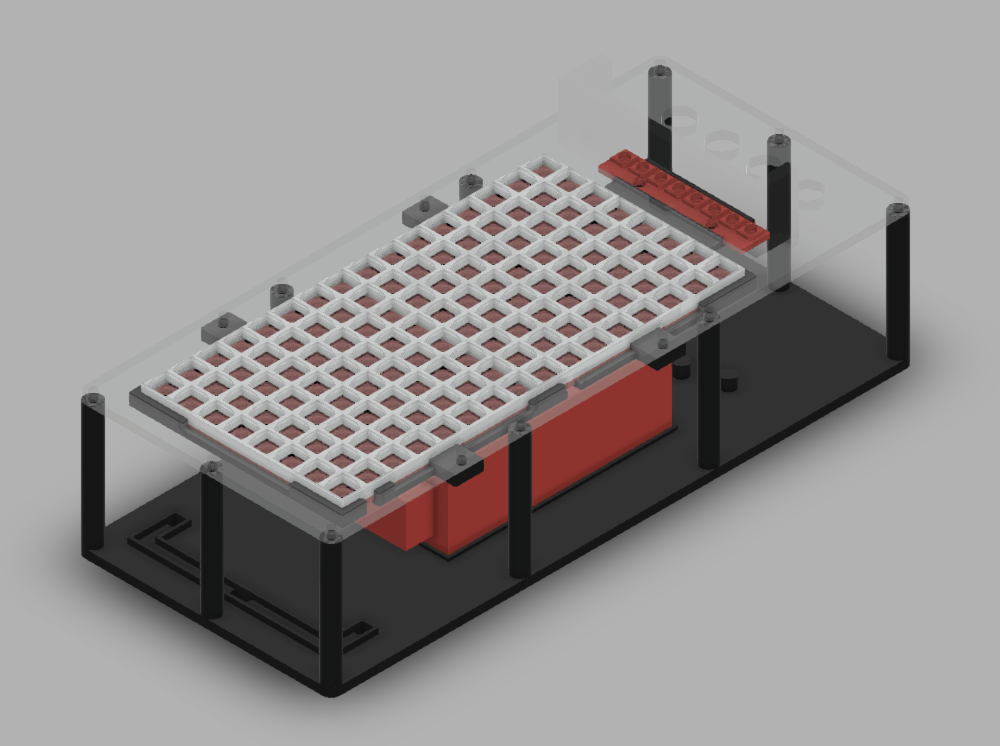
\includegraphics[width=\linewidth,frame]{res/case_render}
        \captionof{figure}{Render of the final product in AutoDesk 360}
        \label{fig:render}
    \end{minipage}}%
    \quad%
    \adjustbox{valign=t}{\begin{minipage}{.45\textwidth}
        \centering
        \adjincludegraphics[
            trim={0 {.48\height} 0 {.1\height}},%
            clip,%
            width=\linewidth,%
            frame%
        ]{res/finished_prototype}
        \captionof{figure}{Final 3D printed prototype}
        \label{fig:prototype}
    \end{minipage}}
\end{figure}
The software for the project is written entirely in Python 3 with JetBrains
IDE PyCharm CE. On the microcontroller board, the code is run by MicroPython,
a small implementation of Python 3 that offers a subset of the Python standard
library and many feature to control lower level hardware components. The case
for the electronic Mastermind was made for the project and is entirely 3D
printed with an Ultimaker printer. Two types of plastic were used for the
print: PLA and PETG.  \par Other software tools were also used.  MobaXTerm is a set
of tools for remote computing, in our case it was used as a serial terminal to
communicate with the microcontroller. AMPY, which stands for Adafruit
MicroPython Tool, allows to write, read and list files that are present in the
MicroPython File System; We used it to upload our code onto the
microcontroller.

\subsection{Design decisions}
Because of some hardware limitations the implementation of Mastermind differs
slightly from the original game. The display has 16 columns so in our version
the Code Breaker has 16 attempts before losing instead of 12.

\subsection{Team organization}
The work was split up in 3 parts: Hardware, Software and Algorithm.
Naoki designed the electrical scheme and a printed circuit board.
Unfortunately, it wasn’t possible to the print it in time for the end of
the week, so we had solder the parts on a prototyping board. Lukas had
to implement the game logic for the microcontroller. And Luke
implemented an algorithm that solves Mastermind in the least possible
number of turns. 

\subsection{Solver algorithm}
The algorithm is composed by two parts. The first part validates the attempts
from the humap players and keep all still possible combinations of colors in a
list. The second part then chooses one of the remainings codes depending on
the situation. We first tried to implement Donald Knuth's algorithm
\cite{knuth} which basically creates a huge tree with the best colors to take
in every situation. But because of the limited memory on the microcontroller
we had to take another less resource expensive approach.  The final version of
our algorithm works by bruteforcing the game. The solution for each step is
computed by running through every color code that is possible and then
comparing the result with other constants.  To decide which combination to try
from its internal list, the following mathematical expression is used.  $$
index = \sqrt{sizeof(list) -1} $$ At the end our algorithm was able to solve
mastermind with an average of 4.82 turns which is nearly as good as the far
more memory consuming alternatives.

\subsection{Software design pattern}
To write the software a pattern called “State-machine” \cite{wikistatepattern}\cite{wikistatemachine} was used
since Mastermind and many other similar games can be represented as a
sequence of states with predetermined actions. A secondary reason is
that State Machines make it easier to add new code to the program. This
design decision comes handy if someone wants to add a new game or
another feature to the project. In our implementation of Mastermind
there are 9 states: {\tt codeSetting, autoCodeSetting, codeGuess,
autoCodeGuess, check,  won, lost, waitingForReset} and {\tt reset}.

% figure
\begin{figure}[H] \centering
    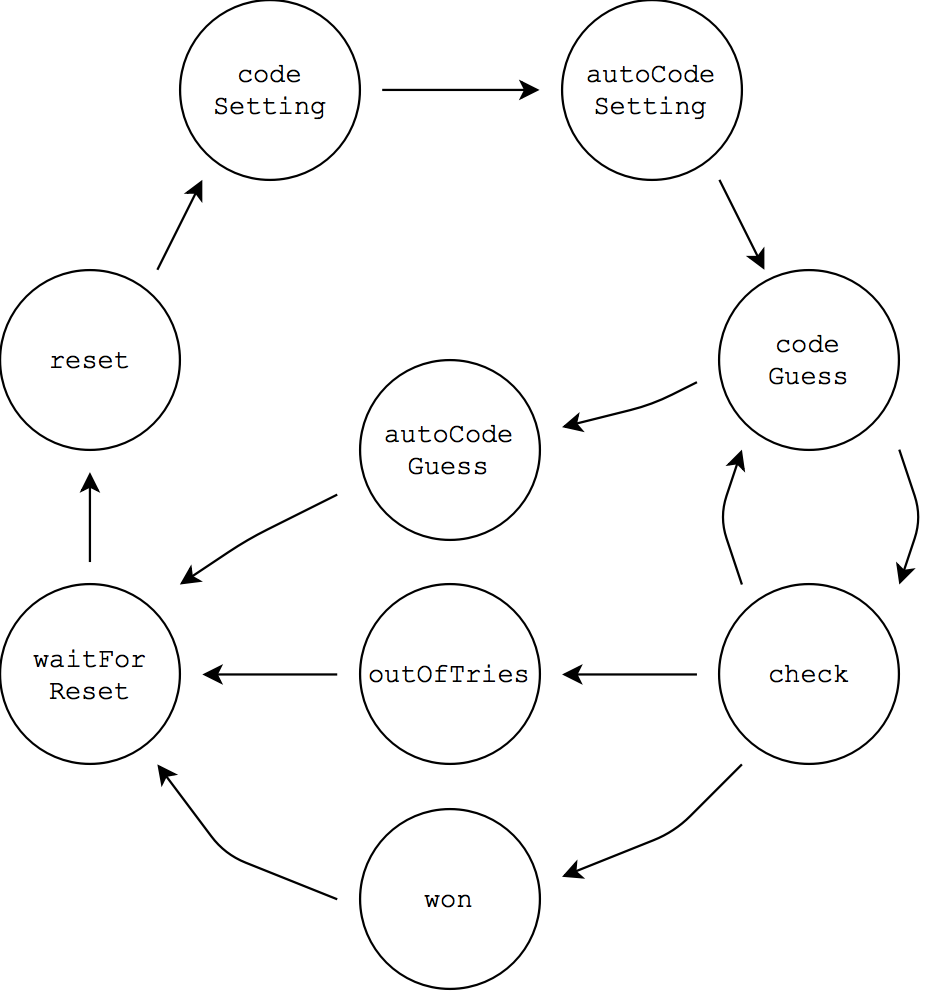
\includegraphics[height=8cm]{res/state_machine}
    \caption{State diagram for the Mastermind code}
\end{figure}
\begin{itemize}

    \item {\tt codeSetting}: Here, the Code Maker sets his code. After
        the Player sets up his code, the program will hide the code and
        switch to the codeGuess state.

    \item {\tt autoCodeSetting}: As mentioned before this state emulates the
        “Code Maker”. It generates 4 random colors for the code for a
        single player mode. As soon as the code is set, the program will
        clear the code and then switch to the {\tt codeGuess} state. This
        state can be entered by pressing button 4 while in {\tt codeSetting}
        state. 

    \item {\tt codeGuess}: Here the codebreaker can try his best to break the
        code. Like in the {\tt codeSetting} state the player can skip through
        the various colors and confirm with the same buttons with the
        exception of button 4 that now works as a game reset. It
        switches to the {\tt reset} state. 

    \item {\tt autoCodeGuess}: This state implements Luke’s algorithm that
        plays the game. It is more a show of than of any use. 

    \item {\tt check}: In this state, the program checks the input from the
        Code Breaker and compares it to the color code of the Code Maker
        and gives a feedback according to the rules. Green means correct
        color and correct place, white means just correct color. After
        this process the the program can switch to either state {\tt won}, if
        all colors are correct and on the right place or state
        {\tt outOfTries}, if the player runs out of attempts. Or if none of
        the previous conditions are met, the state returns to {\tt codeGuess}. 

    \item {\tt won}: This state is simple. It indicates that the Code Breaker
        has won. Then it switches to the state {\tt waitingForReset}.

    \item {\tt outOfTries}: In this case the Code Breaker loses and the Code
        Maker wins. It colors all LEDs in red to indicate a GameOver.
        After that, the program switches to the {\tt waitingForReset} state.

    \item {\tt waitingForReset}: The program simply wait for button 4 to
        be pressed.
        
    \item {\tt reset}: Once this state is called, it resets all variables and
        LEDs and goes back to the {\tt codeSetting} state. 

\end{itemize}

\subsection{Easter egg}
Since we had some spare time the LED Matrix is able to show moving GIFs.
Any image can be uploaded with a GIF to byte array conversion tool we
programmed. The program converts any a 16 by 8 pixels animated GIF file
to an array of frames that contain 3 bytes for each pixel.
This should be a secret state that is only accessible through a secret
color combination while in codeSetting state. When the correct
combination is entered a secret moving low resolution GIF will appear on
the LED Matrix as easter egg.

\section{Results}
In the end, a working Mastermind electronic game prototype was produced.
player 1 can set a color code and player 2 place guesses on how the color code
looks. The system returns a feedback consisting of the amount of correct
placed colors (green) and wrong placed colors (white). There is also a single
player mode implemented where the computer generates a random color-code on
its own. Also a secret feature was implemented. 

\section{Discussion}
\subsection{Technical challenges}
\subsubsection{Debugging}
Debugging the software was difficult because the code was executable
only on the microcontroller due to missing libraries. A software
debugger couldn’t been attached because the program could only run on
the microcontroller. 

\subsubsection{Random number generator}
The random number generator in the ESP32 microcontroller does not
generate pure random numbers. Like in many electronic devices actually
it uses a pseudo random generator function that needs a starting seed
value. To get a truly random value to use as a seed the uptime counter
was used since the measure, in microseconds, depends on the time the
user spends in the {\tt codeSetting} state.

\subsubsection{Memory limitations}
As mentioned before, the platform was intended to implement the auto solve
algorithms. But unfortunately the ESP32 is not able to perform this task
because it does not have enough dynamic memory (RAM) to store the informations
needed to compute the solution. It is still possible to run this code on a
separate program that does not allow to play the game manually.

Some other minor memory related issues were solved by invoking manually the
Micropython garbage collector by using the CPython interface, then ESP32 was
then able to run the program.

\subsection{Hardware failures}
Problems from hardware failures were also present. Originally the
platform controls were intended to be button 1 and button 2 to loop
forward or backward through the colors and button 3 to confirm. But
button 3 suddenly stopped working in the middle of the project, so it
was changed to have button 1 alone to circle through all the various
colors while button 2 confirms the selection.

\section{Acknowledgements}
We especially thank the Swiss Youth in Science that made possible to
organize this great experience. We also want to thank Markus Knecht and
Claude Rubattel for coordinating the study week and our supervisors
Dominik Link, Flavio Müller and Manuel Schlatter for supporting us. Last
but not least we thank the University of Applied Sciences and Arts,
Northwestern Switzerland, School of Engineering for offering the
infrastructure to host the event.

\section*{Softwares}
ESP32 MicroPython Framework: \url{https://github.com/micropython/micropython-esp32} \\
PyCharm IDE: \url{https://www.jetbrains.com/pycharm/} \\
Adafruit MicroPython Tool: \url{https://github.com/adafruit/ampy} \\
MobaXTerm: \url{https://mobaxterm.mobatek.net/}

\begin{thebibliography}{9}
    \setlength\itemsep{0pt}
    \bibitem{mrules}
        \url{http://www.pressmantoy.com/game-rules/Ultimate%20Mastermind%20Rules%20(1).pdf}
    \bibitem{micropythondoc}
        \url{https://docs.micropython.org/en/latest/pyboard/}
    \bibitem{wikistatepattern}
        \url{https://en.wikipedia.org/wiki/State_pattern}
    \bibitem{wikistatemachine}
        \url{https://en.wikipedia.org/wiki/Finite-state_machine}
    \bibitem{knuth}
        \url{http://www.cs.uni.edu/~wallingf/teaching/cs3530/resources/knuth-mastermind.pdf}
    \bibitem{classicmastermind}
        \url{https://my-live-01.slatic.net/p/4/code-breaker-master-mind-mastermind-strategy-board-game-1483679658-39479381-a80c25f5033268e1914a78083757bc07-zoom.jpg}
\end{thebibliography}


\section*{Source code}
The source code and all documents related to the project can be found in
a Git repository hosted on Github at:
\url{https://github.com/flavio99/Mastermind}


\end{document}
